\documentclass[../main.tex]{subfiles}
\begin{document}
\chapter{Caso d'uso: certificazione di OpenStack}
\section{Introduzione}
\textit{OpenStack} è una piattaforma ideata per la realizzazione e la gestione di infrastrutture cloud complesse, pubbliche e private.
Sviluppato inizialmente da \textit{NASA} e \textit{Rackspace}\footnote{Rackspace è una società che opera nell'ambito del cloud-computing con sede a Windcrest, in Texas - \textit{http://www.rackspace.com/}}, è oggi amministrato dalla \textit{OpenStack Foundation}\footnote{La \textit{OpenStack Foundation} è un'organizzazione senza scopo di lucro che promuove lo sviluppo, la distribuzione e l'adozione del progetto \textit{OpenStack}. La fondazione conta più di 18,000 membri individuali da 140 nazioni in tutto il mondo \cite{OpenstackFoundation}. \textit{https://www.openstack.org/foundation/} }, rilasciato sotto licenza Apache\footnote{La licenza Apache è una licenza di software libero, compatibile con la versione 3 della GNU GPL, non copyleft scritta dalla Apache Software Foundation (ASF). Obbliga gli utenti a preservare l'informativa di diritto d'autore e d'esclusione di responsabilità nelle versioni modificate. \textit{http://directory.fsf.org/wiki/License:Apache2.0}} e sostenuto da aziende del calibro di \textit{IBM}, \textit{Cisco}, \textit{Citrix}, \textit{Dell}, \textit{Oracle} e \textit{Red Hat} \cite{OpenstackWhatIs}.

\`E composto da una serie di progetti che si occupano dell'amministrazione delle risorse seguendo il paradigma \textit{infrastructure-as-a-service}; fornisce quindi strumenti per gestire \textit{pool} di macchine virtuali, \textit{storage} e risorse di rete all'interno di un \textit{data-center} cloud.
Il progetto è \textit{open-source} ed è interamente realizzato utilizzando il linguaggio \textit{Python}, seguendo un'architettura totalmente modulare; ogni componente è indipendente dagli altri e può vivere anche in modalità \textit{stand-alone}.
I vari produttori solitamente producono delle derivazioni della piattaforma \textit{OpenStack}, che si differenziano tra loro per la metodologia di automazione del \textit{deployment} dei componenti e dal parco servizi offerto. Una di queste metodologie di automazione è rappresentata da \textit{DevStack} (\textit{http://docs.openstack.org/developer/devstack/}), distribuzione di \textit{OpenStack} orientata allo sviluppo e al testing.

\textit{OpenStack} è strutturato secondo un approccio \textit{multi-tenant}, ed offre un livello di astrazione tale da riuscire a garantire molte delle proprietà di sicurezza descritte nel primo capitolo.
I sorgenti sono disponibili nel repository GitHub \textit{https://github.com/openstack/} .
\paragraph{}
Nell'ambito del progetto di tesi è stato utilizzato \textit{DevStack} in configurazione \textit{all-in-one}\footnote{All in one: tenendo tutti i componenti su un'unica macchina} come riferimento per implementare velocemente alcune delle proprietà di sicurezza su cui sono stati effettuati i test.
In una fase successiva è stato effettuato il \textit{deploy} manuale di un'infrastruttura più complessa distribuita su cinque nodi.

\subsection{Componenti di \textit{OpenStack}}
Tutti i componenti sono implementati come servizi, che espongono delle API \textit{REST}, invocabili tramite un'interfaccia a riga di comando o la \textit{dashboard} grafica \textit{Horizon}.
Grazie alla struttura fortemente modulare e alla natura di software \textit{open-source}, chiunque può sviluppare un proprio componente seguendo le linee guida della \textit{OpenStack Foundation} \cite{GuidelinesOpenstackHacking}.
La comunità \textit{OpenStack} ha comunque identificato una serie componenti che costituiscono il nucleo dell'intera piattaforma, essi sono considerati parte integrante del progetto e vengono perciò mantenuti ufficialmente dalla comunità stessa.
\begin{figure}[H]
\centering
\makebox[\textwidth]{
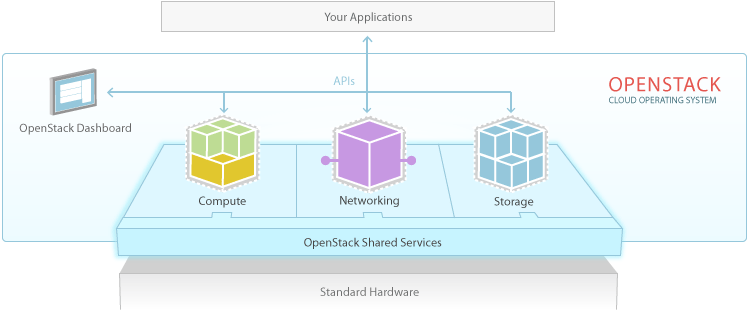
\includegraphics[width=\textwidth]{immagini/openstack-software-diagram.png}
}
\caption{Struttura della Piattaforma OpenStack \cite{OpenstackDiagram}}\label{openstacksw}
\end{figure}
\subsubsection{Identity service: Keystone}
\textit{Keystone} è il componente di \textit{service-catalog}, che si occupa anche di fornire i servizi di gestione delle identità, dei \textit{token} e delle politiche per l'uso specifico dei progetti nella famiglia \textit{OpenStack}.
\`E l'implementazione della "\textit{Identity API}" e ha funzionalità di autenticazione basata su token (\textit{authN\footnote{AuthN: authentication}}) e meccanismi di autorizzazione di alto livello (\textit{authZ}\footnote{AuthZ: authorization}).
\`E stato recentemente ristrutturato per essere espandibile e supportare meccanismi \textit{AuthN/AuthZ} come \textit{OAuth\footnote{Il framework di autorizzazione OAuth permette alle applicazioni di terze parti di ottenere l'accesso con privilegi limitati ai servizi basati su HTTP \cite{OAuth}.}}, \textit{SAML\footnote{SAML, Security Assertion Markup Language, fornisce un framework basato su XML per creare e scambiare online le informazioni sulla sicurezza di un servizio tra due partner \cite{SAML}.}} e \textit{OpenID\footnote{OpenID è un modo sicuro, veloce e facile per fornire un servizio di \textit{single-sign-on} tra siti web \cite{OpenID}.}}.
Nella pratica, si occupa di validare le credenziali degli utenti e dei servizi, rilasciare e gestire i \textit{token} di autenticazione dopo la verifica delle credenziali e di gestire il catalogo dei servizi tenendo traccia dei relativi \textit{endpoint} e dei livelli di autorizzazione ad essi associati.
Supporta numerosi \textit{identity provider} di \textit{back-end}. L'implementazione più comune prevede l'utilizzo di MySQL per la memorizzazione dei ruoli, delle credenziali e delle sessioni, ma è possibile strutturare architetture federate tramite LDAP\footnote{Lightweight Directory Access Protocol, RFC 4510 - \textit{https://tools.ietf.org/html/rfc4510}} o meccanismi di \textit{single-sign-on}\footnote{Si parla di sistema basato su “Single Sign On” (SSO) quando le richieste di autenticazione non vengono direttamente gestite dal sistema stesso ma vengono ridirette verso un’altro sistema di autenticazione che ha precedentemente certificato le credenziali dell’utente connesso, senza quindi avere la necessità di richiedere nuovamente le credenziali per l’accesso \cite{SSO}.}.

\paragraph{Concetti fondamentali}

\subparagraph{Utente}
Rappresentazione digitale di un utente, sistema, servizio che utilizza \textit{OpenStack}.
Se è un utente ad effettuare la richiesta a \textit{Keystone} (e l'autenticazione ha esito positivo), il servizio rilascia un \textit{token} per effettuare le varie richieste.
Gli utenti hanno delle credenziali di \textit{login}, oppure dei \textit{token} per accedere alle risorse.
Possono essere direttamente assegnati ad uno o più progetti (\textit{tenant}), che costituiscono un ambiente isolato (\textit{tenant-isolation}) \cite{KeystoneConcepts}.
\subparagraph{Credenziali}
Dati che confermano l'identità dell'utente (es: nome utente e password, nome utente e chiave API, \textit{token} di autenticazione) \cite{KeystoneConcepts}.
\subparagraph{Autenticazione}
Processo utilizzato per confermare l'identità di un utente, in base alle credenziali fornite.
Una volta avvenuta l'autenticazione, si procede con il rilascio di un token che verrà poi utilizzato per tutte le richieste a seguire \cite{KeystoneConcepts}.
\subparagraph{\textit{Token}}
Stringa alfanumerica utilizzata per accedere alle API di \textit{OpenStack} e alle risorse. Può essere revocato in qualunque momento, ed è valido per un periodo definito \cite{KeystoneConcepts}.
\subparagraph{Progetto o tenant}
Un container utilizzato per raggruppare o isolare le risorse. I tenant isolano anche gli oggetti del servizio di identità.
A seconda delle esigenze, potrebbe corrispondere a un cliente, a un'organizzazione o a un progetto.
\subparagraph{Servizio}
Un servizio di \textit{OpenStack}, come \textit{Nova}, \textit{Swift}, \textit{Glance}. Un servizio è caratterizzato da uno o più \textit{endpoint}, tramite i quali gli utenti possono contattarlo per consultare le risorse da esso custodite ed eseguire le operazioni da esso consentite, nei limiti dei loro privilegi \cite{KeystoneConcepts}.
\subparagraph{\textit{Endpoint}}
Un indirizzo accessibile via rete per contattare un servizio, solitamente è un URL \cite{KeystoneConcepts}.
\paragraph{Ruolo}
Una personalità con un insieme definito di privilegi e diritti, su determinate operazioni.
Il \textit{token} è legato alla lista dei ruoli dell'utente o servizio a cui si riferisce, affinché l'utente possa eseguire tutte le operazioni associate all'insieme aggregato dei ruoli a cui appartiene \cite{KeystoneConcepts}.

\subsubsection{Compute service: Nova}
\textit{Nova} è il componente che si occupa di gestire la parte di Compute di OpenStack. La sua architettura è progettata in un'ottica di scalabilità orizzontale e poggia le sue basi sulle tecnologie di virtualizzazione note. Come hypervisor di backend, infatti, può fare uso di KVM, Xen Server, VMware ed altri.
Le sue funzionalità sono suddivise in vari servizi:
\begin{itemize}
\item \textbf{nova-api}: servizio che si occupa di gestire le richieste di allocazione e gestione delle risorse computazionali effettuate dagli utenti.
Costituisce il cuore dell'interno framework e fornisce la possibilità di controllare l'hypervisor, lo storage e le funzionalità di rete.
Gli endpoint sono servizi HTTP che gestiscono le varie funzioni utilizzando vari tipi di interfaccia (Amazon, Rackspace) e i relativi modelli. Ciò permette alle API di interagire con strumenti già esistenti creati da altri provider.
In un'architettura multi-nodo questo servizio viene installato ed eseguito sul nodo \textit{Controller}.
\item \textbf{nova-scheduler}: si occupa di effettuare lo scheduling delle operazioni invocate da nova-api. Funziona per mezzo di una coda, ed è in grado di individuare il nodo di Compute sul quale deve essere effettuato il deploy delle varie istanze virtuali. Aggiunge dunque un livello di astrazione al fine di consentire la scalabilità orizzontale. Anche questo servizio, nel caso di setup multi-nodo, viene eseguito sul nodo \textit{Controller}.
\item \textbf{Coda di messaggi}, attraverso la quale è orchestrata l'interazione tra i nodi di compute, il controller di rete, le API, lo scheduler e gli altri componenti.
I vari worker leggono cosantemente la coda in base al loro ruolo o, per esigenze specifiche, al loro hostname.
Quando arriva un task sulla coda, il worker ad esso demandato lo esegue e rimanda indietro la risposta, portando il feedback all'utente o servizio che ha generato la richiesta iniziale.
\item \textbf{nova-compute}: è un worker che interagisce con le API dell'hypervisor per creare, eliminare, modificare le varie istanze e le risorse ad esse assegnate. Questo servizio viene generalmente eseguito sullo stesso nodo dell'hypervisor.
Si occupa di:
\begin{itemize}
\item Avviare istanze
\item Terminare istanze
\item Riavviare istanze
\item Agganciare un volume a un'istanza
\item Sganciare un volume da un'istanza
\item Ottenere l'output della console
\end{itemize}
\item \textbf{nova-network}: è il controller di rete. Si occupa principalmente di amministrare le risorse di rete sui vari host. Si occupa di:
\begin{itemize}
\item Allocare indirizzi IP fissi
\item Configurare le VLAN dei vari progetti o tenant
\item Configurare la rete sui nodi di compute
\end{itemize}
Nelle release più recenti di Openstack, \textit{nova-network} è stato sostituito da un servizio dedicato: \textit{neutron}.
\item \textbf{nova-rootwrap}: consente di interagire con le API dell'hypervisor in modo sicuro, senza essere \textit{root} sulla macchina dell'hypervisor, sostituendo il comando \textit{sudo}.
\item \textbf{nova-consoleauth, nova-novncproxy, nova-xvpvncproxy}: si occupano di fornire l'accesso KVM\footnote{Keyboard, Video, Mouse} per le macchine virtuali. Solitamente, affinché ciò possa avvenire, sono utilizzati protocolli di desktop remoto come VNC, Spice o RDP, a seconda di quanto supportato dall'hypervisor.
Il deploy di questi servizi avviene generalmente in questo modo
\begin{itemize}
\item Un processo \textit{nova-consoleauth} sul nodo controller.
\item Un processo \textit{nova-novncproxy} o \textit{nova-xvpvncproxy} sullo stesso nodo delle \textit{nova-api} (spesso nodo Controller). La differenza tra i due, è che il primo fa uso di un client basato su HTML5, mentre l'altro sfrutta la tecnologia Java. 
\end{itemize}
Le connessioni alla console, sia che siano fatte in modo diretto, sia attraverso un proxy, passano attraverso le porte TCP comprese tra 5900 e 5999. Il firewall di ogni nodo di compute deve perciò avere la seguente regola:
\begin{python}
-A INPUT -p tcp -m multiport --dports 5900:5999 -j ACCEPT
\end{python}
\end{itemize}

\begin{figure}[H]
\centering
\makebox[\textwidth]{
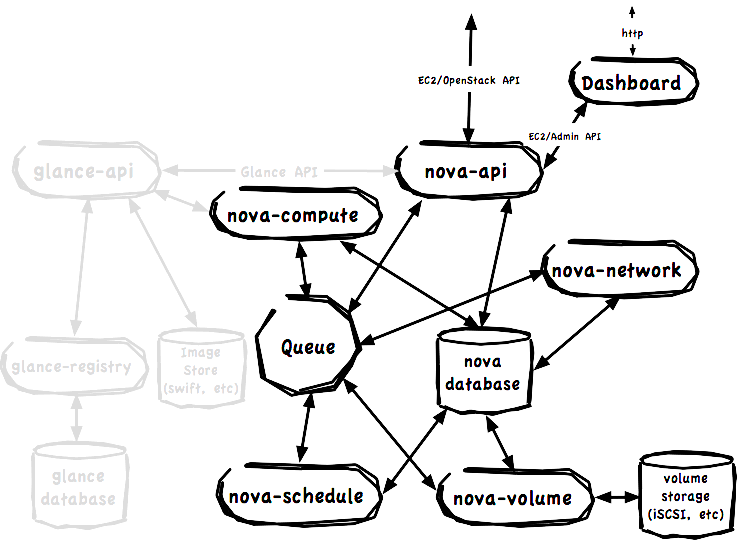
\includegraphics[width=\textwidth]{immagini/nova.png}
}
\caption{Diagramma funzionale di Nova \cite{openstackarch}}\label{openstacknova}
\end{figure}

\subsubsection{Image service: Glance}
\textit{Glance} si occupa della conservazione e la registrazione delle immagini di base per istanziare nuove macchine virtuali.
Il servizio espone un'interfaccia REST che consente di:
\begin{itemize}
\item reperire i metadati relativi a un'immagine
\item caricare una nuova immagine e registrare i relativi metadati
\item scaricare un'immagine in locale
\end{itemize}
Glance fornisce la possibilità di memorizzare le immagini in varie locazioni. Esse possono infatti essere dei semplici file sul disco fisso del nodo su cui Glance è stato eseguito, oppure altri tipi di storage come Swift (il servizio di object-storage).
Esso è scritto secondo i seguenti principi:
\begin{itemize}
\item Architettura componibile
\item Alta disponibilità e scalabilità
\item Tolleranza ai guasti
\item Recuperabilità
\item Utilizzo di tecnologie standard aperte
\end{itemize}
\begin{figure}[H]
\centering
\makebox[\textwidth]{
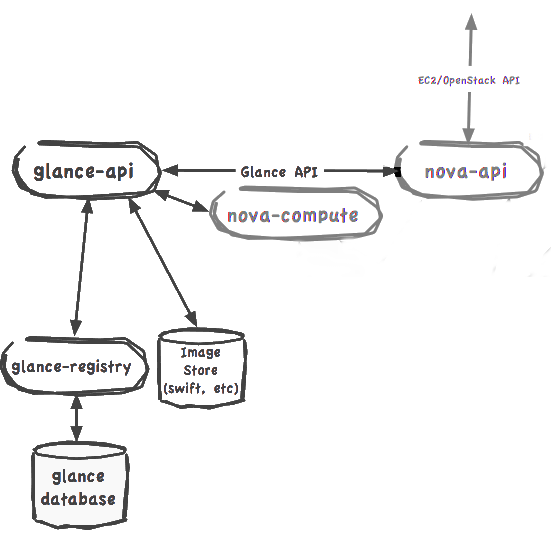
\includegraphics[scale=0.6]{immagini/glance.png}
}
\caption{Diagramma funzionale di Glance \cite{openstackarch}}\label{openstackglance}
\end{figure}


\subsubsection{Networking service: Neutron}
\textit{Neutron} è il componente di OpenStack che offre il servizio di "networking as a service" per le macchine virtuali, effettuando un'astrazione del livello di rete.
Lo scopo è principalmente quello di fornire delle API per strutturare la rete in modo avanzato e costruire topologie complesse, dotate di politiche di networking eterogenee.
Affinché ciò possa avvenire, Neutron fa uso di tecnologie di software-defined networking, come OpenFlow e Open-vSwitch, incapsulando il traffico con varie tecnologie di tunneling come VXLAN e GRE.
\`E strutturato su un'architettura totalmente componibile tramite plug-in, che possono essere sia open-source che proprietari, i quali forniscono le modalità per amministrare in modo efficiente le capabilities di rete.
La filosofia è quindi quella di implementare l'approccio \textit{as-a-service} anche per il livello di rete, al fine di fornire le seguenti funzionalità:
\begin{itemize}
\item Load balancer-aaS
\item VPN\footnote{Virtual Private Network}-aaS
\item Firewall-aaS
\item IDS-aaS
\item etc.
\end{itemize}
Un'altra funzionalità introdotta da Neutron, è quella di creare molteplici reti virtuali e di garantire la tenancy isolation agendo direttamente sul livello 2 dello stack ISO/OSI
Le API forniscono inoltre numerosi livelli di controllo per:
\begin{itemize}
\item Politiche di sicurezza e \textit{compliance}
\item Qualità del servizio
\item Monitoraggio e risoluzione dei problemi
\end{itemize}

%http://www.slideshare.net/danwent/openstack-quantum-intro-os-meetup-32612

\begin{table}[h]
\centering
\begin{tabular}{| m{3cm}| m{5cm} | m{5cm} | }
\hline
& \textbf{Nova} & \textbf{Neutron} \\ \hline
\textit{*-as-a-service} & Compute & Network \\ \hline
\textit{Livello di astrazione} & \textbf{server virtuali}, rappresentano host con una CPU, della RAM, dischi e interfacce di rete & \textbf{reti virtuali}: segmenti di livello 2, \textbf{porte virtuali}: punti di aggancio per i dispositivi connessi alle reti virtuali \\ \hline
\textit{Tecnologie di backend supportate} & libvirt per KVM, XenServer, Hyper-V, vMware ESX & Open vSwitch, Cisco UCS, Linux Bridge \\ \hline
\textit{Espandibilità delle API} & \textit{keypair}, ripristino delle istanze, volumi, etc. & \textit{QoS}, statistiche sulle porte, \textit{security groups}, etc. \\ \hline

\end{tabular}
\caption{Analogie tra Neutron e Nova}
\label{tab:AnalogiesNeutronNova}
\end{table}
\begin{figure}[H]
\centering
\makebox[\textwidth]{
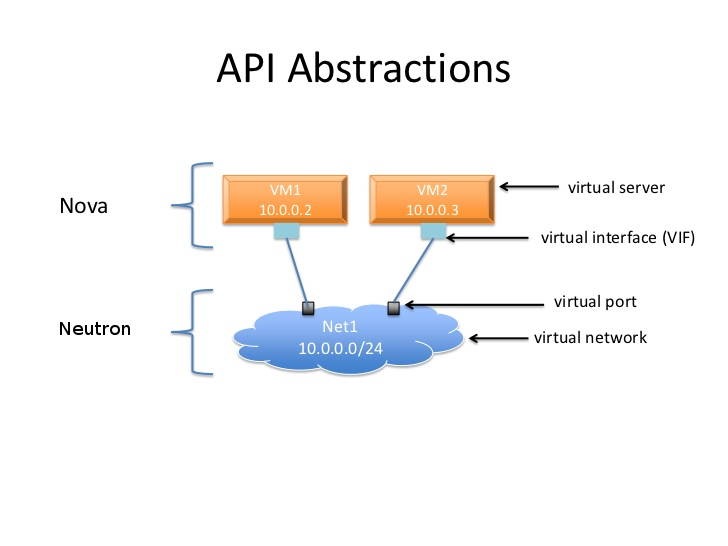
\includegraphics[width=10cm]{immagini/neutronNova.jpg}
}
\caption{Astrazione delle API di Neutron\cite{NeutronNova}}\label{NeutronNova}
\end{figure}

\subsubsection{Object-storage service: Swift}
Swift è un sistema di storage di oggetti distribuito e orientato a configurazioni in alta disponibilità.
L'approccio "\textit{object-storage}" tratta i dati come oggetti binari \textit{blob} - 
Gli oggetti vengono memorizzati e referenziati generalmente tramite il protocollo HTTP, mappando in modo RESTful le azioni CRUD.
Nel caso di Swift, gli oggetti sono fisicamente memorizzati su "\textit{object-servers}".
Più "\textit{object-servers}" formano un \textit{ring}, il quale rappresenta il componente unitario per l'erogazione del servizio Swift.
Per memorizzare le informazioni relative a un oggetto, viene mantenuto un catalogo basato su metadati.
Affinché sia possibile fornire proprietà di resilienza, i \textit{rings} possono essere divisi in zone, nelle quali i dati vengono replicati in caso di guasti hardware.
Le zone possono essere rappresentate da un singolo hard disk, un server o un dispositivo presso un datacenter esterno (che può avere ulteriori meccanismi di replica).
Per la configurazione predefinita vengono create tre repliche di ogni dato, ognuna delle quali viene memorizzata in una zona separata.
L'operazione di replica avviene in modo asincrono, ma può fallire o venire sospesa nel caso in cui il server venga spento o scollegato dall'infrastruttura o l'infrastruttura sia sottoposta a carichi elevati.
Per questo motivo potrebbero verificarsi casi di inconsistenza dei dati.

\subsubsection{Block-storage service: Cinder}
\textit{Cinder} è un servizio che fornisce la possibilità di centralizzare la gestione e la creazione di volumi di storage organizzazi a blocchi.
Nello scenario più comune, i volumi Cinder rappresentano lo storage persistente alle istanze.
Cinder permette di eseguire le operazioni di base per la gestione dei volumi di storage, di espandere i volumi, di gestirne gli snapshot (i volumi sono incapsulati in file) e clonarli.
Permette inoltre di fornire un catalogo di dispositivi di storage con caratteristiche differenti (\textit{volume-types}), che possono implementare o meno determinate feature (ad es. crittografia con LUKS).
Il dispositivo di storage fisico, sia esso un disco (o un pool di dischi) magnetico o a stato solido, può essere localizzato all'interno dei server Cinder, oppure su un'architettura di storage esterna (SAN) resa disponibile ai nodi Cinder e agli hypervisors tramite canali iSCSI, NFS o Fibre Channel.
Soluzioni alternative supportate in questo senso, prevedono l'utilizzo di software come GlusterFS o RDB.

\subsubsection{Altri servizi}
Altri componenti di OpenStack sono
\begin{itemize}
\item{Database service: Trove}
\begin{Verbatim}[frame=single]
https://wiki.openstack.org/wiki/Trove
\end{Verbatim}
\item{Orchestration service: Heat}
\begin{Verbatim}[frame=single]
https://wiki.openstack.org/wiki/Heat
\end{Verbatim}
\item{Bare-metal provisioning service: Ironic}
\begin{Verbatim}[frame=single]
https://wiki.openstack.org/wiki/Ironic
\end{Verbatim}
\item{Data-processing service: Sahara}
\begin{Verbatim}[frame=single]
https://wiki.openstack.org/wiki/Sahara
\end{Verbatim}
\item{Messaging service: Zaqar}
\begin{Verbatim}[frame=single]
https://wiki.openstack.org/wiki/Zaqar
\end{Verbatim}
\item{Key management service: Barbican}
\begin{Verbatim}[frame=single]
https://wiki.openstack.org/wiki/Barbican
\end{Verbatim}
\item{DNS service: Designate}
\begin{Verbatim}[frame=single]
https://wiki.openstack.org/wiki/Designate
\end{Verbatim}
\item{Shared Filesystem service: Manila}
\begin{Verbatim}[frame=single]
https://wiki.openstack.org/wiki/Manila
\end{Verbatim}
\item{Application catalog service: Murano}
\begin{Verbatim}[frame=single]
https://wiki.openstack.org/wiki/Murano
\end{Verbatim}
\item{Governance service: Congress}
\begin{Verbatim}[frame=single]
https://wiki.openstack.org/wiki/Congress
\end{Verbatim}
\item{Workflow service: Mistral}
\begin{Verbatim}[frame=single]
https://wiki.openstack.org/wiki/Mistral
\end{Verbatim}
\item{Key-value store \textit{as-a-service}: MagnetoDB}
\begin{Verbatim}[frame=single]
https://wiki.openstack.org/wiki/MagnetoDB
\end{Verbatim}
\end{itemize}


\subsection{Componenti di supporto}
\subsubsection{Dashboard: Horizon}
Horizon è l'interfaccia grafica del progetto OpenStack.
Si tratta di una web-app sviluppata in Python 2.7 con framework Django, espandibile tramite vari plug-in per consentire l'integrazione con i vari componenti di OpenStack (tramite API REST).


Non è studiata nell'ottica dell'amministrazione dell'infrastruttura cloud, quanto nell'intenzione di fornire all'utente finale una dashboard per eseguire le operazioni più semplici. Per questo motivo molte funzionalità utilizzabili tramite riga di comando non sono integrate in Horizon.
Permette comunque agli amministratori di usufruire di un'interfaccia grafica di reporting sullo stato dell'infrastruttura (in termini di utilizzo della stessa, di risorse allocate e di risorse disponibili) e di effettuare operazioni ordinarie come la gestione delle utenze e dei progetti.
\begin{figure}[H]
\centering
\makebox[\textwidth]{
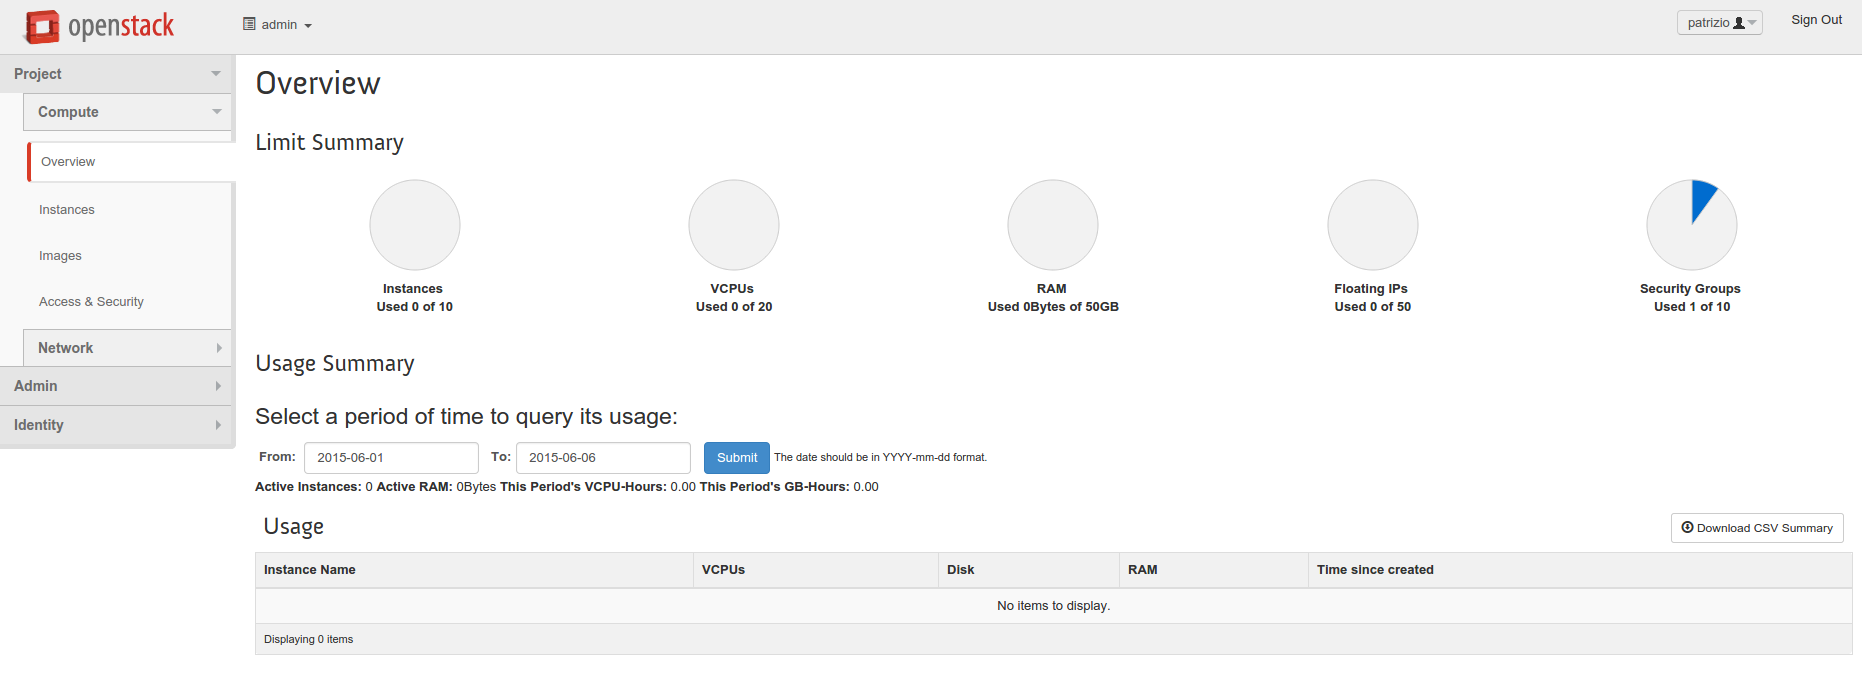
\includegraphics[width=\textwidth]{immagini/Horizon.png}
}
\caption{Horizon - Dashboard}\label{HorizonImg}
\end{figure}
\subsubsection{Telemetry-service: Ceilometer}
Poiché OpenStack fornisce il servizio \textit{Infrastructure-as-a-Service} ai clienti, è spesso necessario essere in grado di misurarne l'utilizzo e le performance per stabilire metriche di fatturazione, benchmarking, scalabilità e scopi statistici.
Ceilometer è il servizio di metering più promettente e maturo per l'infrastruttura OpenStack. 
Il suo nome deriva dall'ambito metereologico: il nefoipsometro (ceilometer) è infatti un dispositivo ottico, a ultrasuoni o laser, in grado di calcolare l'altezza dello strato nuvoloso nel cielo.
Per analogia, il progetto Ceilometer costituisce un framework per il monitoraggio e la misurazione di OpenStack.
Gli obiettivi di Ceilometer sono i seguenti:
\begin{itemize}
\item Collezionamento efficiente di dati di misurazione in termini di CPU e costi di rete
\item Collezionamento dei dati provenienti dai vari servizi o da attività  di polling
\item Configurazione delle tipologie dei dati collezionati per rispettare vari requisiti operativi
\item Permettere l'accesso e l'inserimento dei dati di metering tramite API REST.
\item Costruzione di un framework espandibile, per collezionare anche dati provenienti da componenti \textit{ad-hoc}, tramite plugin appositamente sviluppati
\item Garantire la non repudiabilità dei dati collezionati tramite meccanismi di firma
\end{itemize}
La struttura di Ceilometer è così composta:
\begin{itemize}
\item Un'interfaccia REST per fornire l'accesso ai dati di metering contenuti nel database
\item Un agente centrale che raccoglie statistiche di utilizzo per le risorse non relative alle istanze o ai nodi di compute.
\item Agenti per i nodi di compute che raccolgono le statistiche dei nodi di compute e delle istanze.
\item Un collettore che controlla la coda dei messaggi (per le notifiche inviate dall'infrastruttura e per i dati di misurazione provenienti dagli agenti).  I messaggi vengono poi processati, firmati e inviati su un unico bus etichettati in modo appropriato. Il collettore può essere eseguito su uno o più server.
\item Un database per memorizzare i dati che sia in grado di gestire scritture (da parte dei collector) e letture concorrenti (da parte delle API REST)
\end{itemize}

Questi servizi comunicano utilizzando il bus predefinito di OpenStack. Solamente il collector e il server delle API hanno accesso al database.
I database supportati sono MongoDB, HBase e tutti i database relazionali  supportati da SQLAlchemy.
In ogni caso in produzione è generalmente raccomandato l'utilizzo di MongoDB,  installato su un server dedicato, poiché offre meccanismi ottimizzati per l'elaborazione di letture e scritture effettuate in modo concorrente.

Le stime di utilizzo del database in un ambiente di produzione sono di 386 scritture per secondo e di circa 33 milioni di eventi al giorno, che richiedono circa 240 GB di storage al mese.

\subsubsection{Testing and benchmarking: Tempest e Rally}
Tempest è la test suite ufficiale di OpenStack. \`E uno strumento che si occupa di eseguire un insieme di test funzionali su un'infrastruttura cluster OpenStack.
Esso esegue automaticamente vari test per ciascuna delle patch in ogni progetto di OpenStack, permettendo all'amministratore dell'infrastruttura di aggiungere funzionalità che introducano malfunzionamenti.

La complessità di Tempest è notevole e potrebbe richiedere molto tempo per essere appreso. Inoltre manca di alcune funzionalità utili per il benchmarking, come la possibilità di effettuare simulazioni di carico e di restituire i risultati graficamente.

La soluzione a questo problema è fornita da un altro componente, Rally, che si occupa della validazione e dei test di benchmark sull'infrasatruttura OpenStack.
Rally automatizza l'installazione, la configurazione e l'esecuzione di Tempest, con la capacità di gestire automaticamente più infrastrutture.

Il motore di benchmarking è inoltre in grado di lavorare con simulazioni di carico e di memorizzare i risultati dei test in un database, favorendo le attività di reporting.
\vfill
\newpage

\section{Ambiente di test all-in-one con Devstack}
\subsection{Cos'è DevStack}
DevStack è un'insieme di script BASH per creare velocemente un ambiente OpenStack completo di tutti i servizi. Non è da considerarsi un installer per OpenStack, è piuttosto uno strumento per creare un ambiente di sviluppo ed effettuare dimostrazioni di funzionamento.
Esso supporta un vasto insieme di configurazioni possibili, integrazioni con varie piattaforme e servizi di supporto.
Essendosi evoluto velocemente, tuttavia, presenta numerose problematiche. Inoltre, molte delle configurazioni supportate, non sono mai state effettivamente testate.
L'obiettivo è dunque quello di fornire e di mantenere gli strumenti per la gestione dei servizi OpenStack sempre alle versioni più recenti, attingendo direttamente dal repository GIT, per fini di sviluppo.
Nell'ambito del progetto di tesi è stato più volte utilizzato per creare gli scenari adatti all'esecuzione di test sulle funzionalità di sicurezza di OpenStack.
\subsection{Deploy di DevStack in configurazione all-in-one}
La configurazione all-in-one di DevStack prevede la presenza di tutti i servizi OpenStack su un'unica macchina.
In questo modo si può usufruire di una configurazione funzionante, comprendente tutti i servizi essenziali, in poco tempo.

I sistemi operativi host sul quale è stato effettuato il deploy di DevStack sono:
\begin{itemize}
\item Fedora 19 e Fedora 20
\item CentOS 6.5 e CentOS 7
\item Ubuntu Server 12.04 e Ubuntu Server 14.04
\end{itemize}

Per eseguire il deploy di devstack è necessario effettuare i seguenti passaggi:
\begin{enumerate}
\item Installare uno dei sistemi operativi sopra elencati
\item Scaricare e installare \textbf{git}:

\textit{Ubuntu:}
\begin{Verbatim}
sudo apt-get install -y git 
\end{Verbatim}
\textit{Fedora:}
\begin{Verbatim}
sudo yum install -y git
\end{Verbatim}
\item Posizionarsi nella cartella \textit{/opt}
\begin{verbatim}
cd /opt
\end{verbatim}
\item Effettuare il download di Devstack dal repository GIT:
\begin{Verbatim}
sudo git clone https://git.openstack.org/openstack-dev/devstack
\end{Verbatim}
\item Creare un utente dedicato all'esecuzione di Devstack. Questa operazione può essere automatizzata tramite il comando:
\begin{Verbatim}
sudo ./devstack/tools/create-stack-user.sh
\end{Verbatim}
Verrà quindi creato un utente \textit{stack}, avente directory home in \textit{/opt/stack}. \`E utile a questo punto impostare una password per l'utente tramite il comando:
\begin{verbatim}
sudo passwd stack
\end{verbatim}
\item Assegnare la ownership della cartella di Devstack all'utente \textit{stack}:
\begin{verbatim}
sudo chown stack:stack /opt/devstack
\end{verbatim}
\item Uscire dalla sessione corrente con il comando \textit{exit} ed effettuare il login con l'utente \textit{stack} e la password impostata precedentemente.
\item Posizionarsi in \textit{/opt/devstack}:
\begin{verbatim}
cd /opt/devstack
\end{verbatim}
\item Creare un file di configurazione chiamato \textit{local.conf} per il deployment. Un esempio può essere trovato in \textit{/opt/devstack/samples/local.conf} così composto:
\begin{python}
[[local|localrc]]
ADMIN_PASSWORD=password_amministratore
DATABASE_PASSWORD=password_db
RABBIT_PASSWORD=password_broker
SERVICE_PASSWORD=password_servizi
SERVICE_TOKEN=a682f596-76f3-11e3-b3b2-e716f9080d50
\end{python}
Se i parametri "\textit{\_PASSWORD}" non vengono specificati, durante il deployment verranno chieste le password in modo interattivo.
La funzionalità del parametro SERVICE\_TOKEN è quella di fornire un meccanismo di autenticazione, nei confronti di Keystone, senza credenziali per l'amministrazione dei servizi. A tale scopo viene generalmente usato un \textit{UUID} generato tramite la libreria \textit{libuuid} con il comando linux \textit{uuidgen}.
Tramite il file \textit{local.conf} è inoltre possibile gestire il deployment dei vari servizi di OpenStack, abilitare il logging, oppure specificare le configurazioni per i vari servizi (es. aumentare la dimensione del file di backend per la gestione dei volumi \textit{Cinder}).
Ulteriori informazioni possono essere trovate all'indirizzo \textit{http://docs.openstack.org/developer/devstack/configuration.html}.
\item Lanciare il comando \textit{./stack.sh}.
Questo comando effettuerà il download di tutte le dipendenze in base a quanto specificato nel file \textit{local.conf}, installerà i vari servizi di OpenStack e li lancerà in una sessione di background gestita tramite il comando \textit{screen}.

Una volta completata la fase di \textit{deployment} verranno riportate le informazioni di accesso:
\begin{verbatim}
Horizon is now available at http(s)://FQDN/
Keystone is serving at http(s)://FQDN:5000/vX.0/
Examples on using novaclient command line is in exercise.sh
The default users are: admin and demo
The password: [PASSWORD]
This is your host ip: [IP]
\end{verbatim}
\end{enumerate}
Per fermare l'esecuzione di Devstack si può usufruire dello script \textit{unstack.sh}. Questo terminerà in modo sicuro tutti i servizi, senza perdita di dati.

Qualora si volesse riavviare Devstack, è possibile utilizzare il comando \textit{rejoin-stack.sh}. Un'eventuale esecuzione di \textit{stack.sh} potrebbe comportare perdite di dati.

In ultimo, il comando \textit{clean.sh}, effettua una pulizia completa del sistema da Devstack, rimuovendo tutti i dati ad esso collegato, disinstallando tutte le dipendenze e riportandolo alle condizioni iniziali.
\subsection{Protezione dei canali di comunicazione con TLS/SSL}
L'interoperabilità tra più nodi di una stessa infrastruttura pone notevoli problematiche dal punto di vista della sicurezza.
\`E importante quindi proteggere il canale di comunicazione, affinché solamente gli \textit{endpoint} possano essere in grado di interpretare i messaggi. Tuttavia la cifratura del canale deve essere applicata solamente come parte di una strategia di sicurezza più avanzata: un eventuale attaccante potrebbe infatti compromettere direttamente gli \textit{endpoint} e avere comunque accesso al contenuto del canale e la capacità di monitorarlo \cite{OpenStackSecurity}.

Al fine di proteggere le API dei vari servizi, OpenStack fa uso della tecnologia \textit{TLS}, precedentemente discussa.
A tal fine si possono utilizzare due strategie:
\begin{enumerate}
\item Implementazione di TLS/SSL sui servizi in modo nativo
\item Utilizzo di proxy TLS/SSL davanti agli endpoint
\end{enumerate}
Dal punto di vista della sicurezza è preferibile adottare la prima soluzione: è buona norma infatti effettuare le operazioni di cifratura il prima possibile e quelle di decifratura il più tardi possibile.
Tuttavia essa non offre grandi prospettive di scalabilità, è di difficile implementazione e non offre la separazione dei privilegi (i servizi di OpenStack hanno accesso diretto alle chiavi private: in caso di compromissione del servizio ciò potrebbe costituire un enorme problema problema).
La seconda, invece, sebbene non soddisfi il principio sopra citato, è di più facile implementazione, offre opportunità di scalabilità e \textit{load-balancing} e permette di effettuare  la separazione dei privilegi \cite{OpenStackSecurity}.
Per implementare la seconda strategia si può fare uso di due modelli:

\begin{itemize}
\item SSL/TLS sulla stessa macchina fisica degli endpoint
\begin{figure}[H]
\centering
\makebox[\textwidth]{
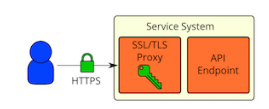
\includegraphics[width=5cm]{immagini/SSLPhys.png}
}
\caption*[Proxy SSL/TLS sulla stessa macchina fisica \cite{OpenStackSecurity}]{}\label{SSLPhys}
\end{figure}


\item Proxy SSL/TLS esterno, posto davanti all'endpoint
\begin{figure}[H]
\centering
\makebox[\textwidth]{
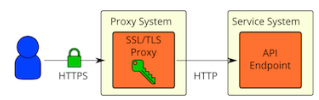
\includegraphics[width=5cm]{immagini/SSLInFront.png}
}
\caption*[Proxy SSL/TLS esterno \cite{OpenStackSecurity}]{}\label{SSLInFront}
\end{figure}
\end{itemize}

Nella prima casistica il servizio resta in ascolto sull'interfaccia di \textit{loopback}, e viene posto un proxy in ascolto sull'interfaccia pubblica. In questo modo tutte le comunicazioni devono essere obbligatoriamente veicolate sul proxy ed avvengono in modo sicuro; viene inoltre fatta la separazione dei privilegi demandando la gestione della chiave privata al servizio proxy.
Nella seconda casistica, invece, il servizio proxy è posto su un host esterno e si occupa di filtrare uno o più endpoint dei servizi Openstack. Ciò consente la realizzazione di infrastrutture scalabili e di effettuare load-balancing, per la realizzazione di infrastrutture ad alta disponibilità.

Inoltre è possibile separare le tecniche crittografiche tra l'ambiente esterno e l'ambiente interno.
Un fornitore di servizi cloud pubblico, per esempio, potrebbe voler esporre le API pubbliche con un determinato certificato, magari riconosciuto da una \textit{Certification Authority} root fidata, ed utilizzare la propria \textit{PKI}\footnote{Pubic Key Infrastructure} per gestire la comunicazione tra i servizi interni.
Questa separazione può essere effettuata decrittando i dati sul canale tra proxy e client,
e iniziando una nuova sessione verso gli endpoint di OpenStack crittografando i dati con le nuove chiavi.
C'è un breve momento, in questo caso, in cui i dati sono in chiaro, ma si suppone che essi non vengano trasmessi nuovamente sulla rete se non in modo cifrato, per cui non sussiste alcuna problematica di sicurezza.
In questo caso, tuttavia,  La compromissione dell'host che offre il servizio proxy potrebbe costituire una minaccia.
\begin{figure}[H]
\centering
\makebox[\textwidth]{
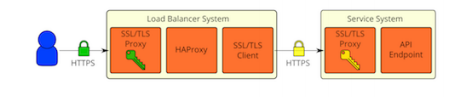
\includegraphics[width=9cm]{immagini/SSLSep.png}
}
\caption{Separazione della crittografia \cite{OpenStackSecurity}}\label{SSLSep}
\end{figure}

Al fine di effettuare alcune tipologie di test è stato necessario predisporre Devstack per l'utilizzo della cifratura sul canale di comunicazione.
A tal fine, si è collaborato alla realizzazione della patch 98854 "\textit{Configure endpoints to use SSL natively or via proxy}"\footnote{Configure endpoints to use SSL natively or via proxy
 - https://review.openstack.org/\#/c/98854/} di Rob Crittenden, la quale è stata recentemente integrata ufficialmente nel progetto.

Grazie a questa patch, Devstack supporta entrambe le modalità descritte: è possibile sia orchestrare la configurazione di un proxy SSL Apache, sia utilizzare direttamente SSL sugli endpoint dei servizi OpenStack. Sono supportati \textit{nova}, \textit{cinder}, \textit{glance}, \textit{swift} e \textit{neutron}.
Devstack si occupa di generare automaticamente tutti i certificati e di caricare le Certification Authority nell'elenco delle autorità fidate su tutti i nodi coinvolti nel deployment.
Alternativamente è possibile specificare dei certificati e delle chiavi di cifratura già presenti.

Per abilitare la funzionalità di proxy TLS sull'endpoint è sufficiente inserire nel file \textit{local.conf} la direttiva:
\begin{python}
ENABLED_SERVICES+=,tls-proxy
\end{python}

Invece, per abilitare SSL in modalità nativa è sufficiente specificare:
\begin{python}
USE_SSL=True
\end{python}

Per utilizzare dei certificati generati precedentemente al deployment occorre specificare le variabili:
\begin{python}
<SERVICE>\_SSL_CERT=/percorso/del/certificato
<SERVICE>\_SSL_KEY=/percorso/della/chiave/privata
<SERVICE>\_SSL_PATH=/percorso/della/certification/authority
\end{python}
sostituendo a \textit{<SERVICE>} il nome del servizio.
\`E buona norma, inoltre, impostare la variabile \textit{SERVICE\_HOST} all'FQDN dell'host. Il valore di default di questa variabile è l'indirizzo IP della prima interfaccia di rete fisica individuata.
La patch non imposta SSL sull'endpoint di Horizon, che viene servito per configurazione predefinita tramite Apache con supporto WSGI.
\`E tuttavia possibile agire manualmente sul file di configurazione del Virtual Host per fornire HTTPS anche sulla dashboard.
\vfill
\section{Ambiente di test multi-nodo}
L'esecuzione dei test descritti nei paragrafi a seguire ha portato alla necessità di realizzare un'infrastruttura OpenStack multinodo presso il laboratorio SESAR.
Il deployment di questa infrastruttura ha consentito l'esecuzione del framework in un contesto più simile a un ambiente reale di produzione.
La struttura dell'infrastruttura è raffigurata nella Figura \ref{SesarStack}
\begin{figure}[H]
\centering
\makebox[\textwidth]{
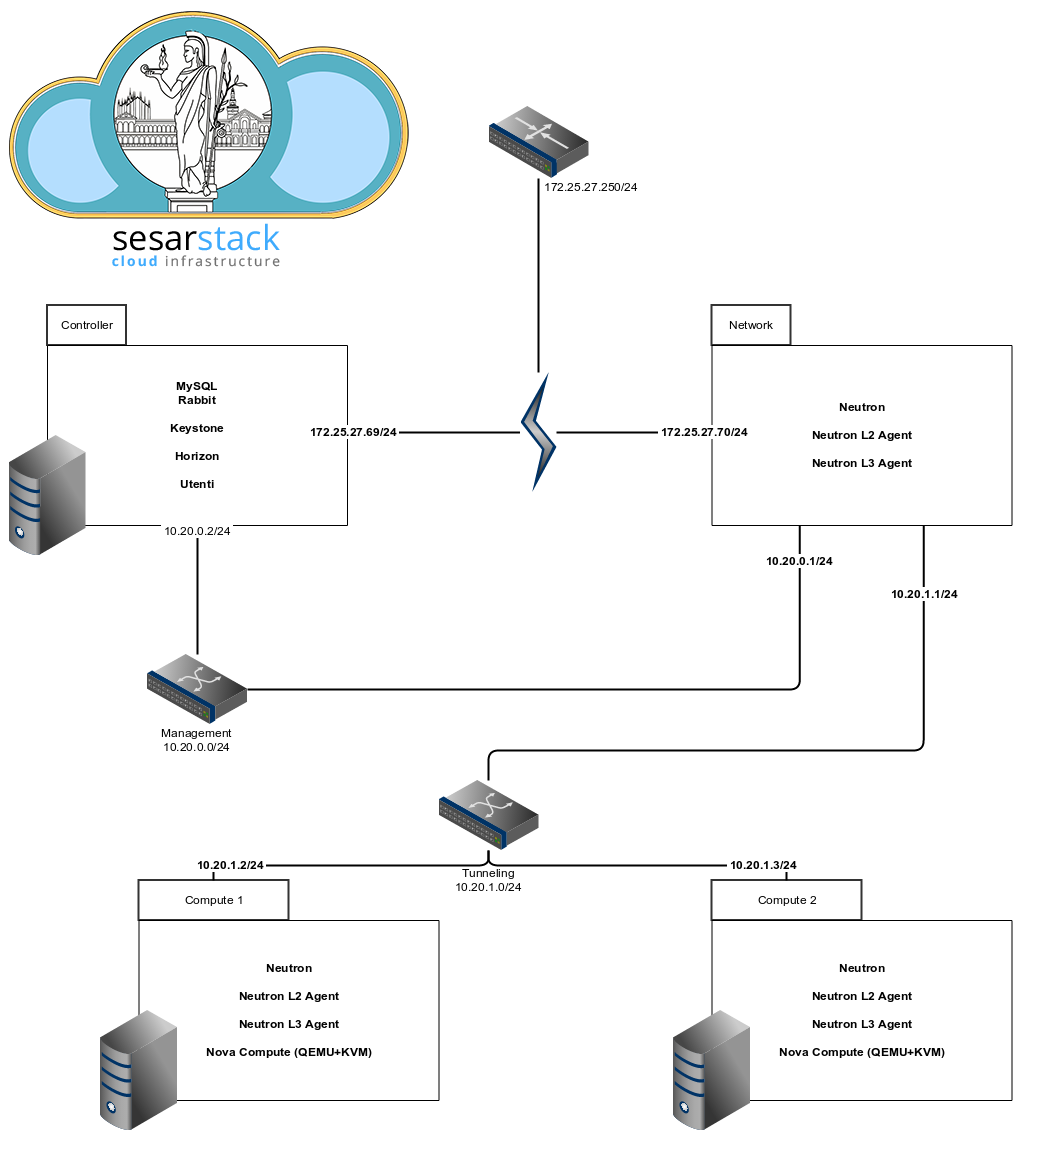
\includegraphics[width=\textwidth]{immagini/sesarstack.png}
}
\caption{Struttura Sesar Stack}\label{SesarStack}
\end{figure}
Sono state allestite due reti gestite da due switch a livello due ISO/OSI:
\begin{itemize}
\item Rete di management, che collega tutti gli host
\item Rete di tunneling, che collega esclusivamente i nodi di Compute al nodo di rete, sulla quale si appoggia lo stack di rete software-defined gestito da Open vSwitch.
\end{itemize}
Successivamente è stato effettuato il deploy di Red Hat OpenStack su quattro nodi, con sistema operativo CentOS 7, così organizzati:
\begin{itemize}
\item 1 Controller - Horizon, Nova, Keystone, connesso alla rete di laboratorio (172.25.27.0/24), con collegamento Internet,  e alla rete di \textit{Management}
\item 1 Network - Neutron L2, Neutron L3, connesso alla rete di laboratorio, alla rete di Management e alla rete di \textit{Tunneling}
\item 2 Compute - Nova, Neutron L2, Neutron L3, connessi alla rete di \textit{Management} e alla rete di \textit{Tunneling}
\end{itemize}

La \textit{sonda} sviluppata come progetto di tesi è stata poi posizionata sia a livello infrastruttura (in modalità \textit{bare-metal}, con Raspberry PI), che come macchina virtuale, per eseguire i test a livello \textit{PaaS} e \textit{SaaS}.
\section{Certificazione della sicurezza e valutazione dei costi}
\paragraph{Studio della sicurezza di OpenStack}
La OpenStack Foundation ha formato un gruppo chiamato \textit{OSSG} (\textit{OpenStack Security Group}), responsabile di:
\begin{itemize}
\item Creare e mantenere un documento contenente le linee guida per la sicurezza \cite{OpenStackSecurity}
\item Tenere traccia delle vulnerabilità sulla piattaforma
\end{itemize}
Il team OSSG ha identificato quattro principali domini di sicurezza:
\begin{itemize}
\item \textit{Pubblico}: riguarda la partizione non fidata dell'infrastruttura cloud. Ogni dato  con requisiti di confidenzialità e integrità, deve essere opportunamente protetto prima di transitare nel dominio pubblico.
\item \textit{Guest}: riguarda le comunicazioni tra le istanze o tra le applicazioni ospitate dall'infrastruttura.
\item \textit{Gestione}: riguarda le comunicazioni e i dati  prodotti dagli strumenti e i servizi fondamentali per il funzionamento dell'infrastruttura cloud (es. OpenStack)
\item \textit{Dati}: riguarda le informazioni a proposito dei servizi di memorizzazione dei dati di OpenStack (es. Glance, Cinder, nova-volume, Swift).
\end{itemize}
Nei paragrafi seguenti vengono mostrati i criteri per la validazione del framework proposto e del componente sviluppato, applicandolo a uno specifico caso d'uso: la certificazione di OpenStack.
La valutazione del framework è fondata sulla corrispondenza tra i servizi \textit{core} di OpenStack e i domini di sicurezza sopra descritti (figura \ref{fig:OpenStackServiziDomini}), e si basa sul lavoro di \textit{Anisetti et al.} nella pubblicazione "\textit{Toward Security and Performance Certification of OpenStack}" \cite{CertOpenstack}.


\begin{figure}[H]
\centering
	\resizebox{\textwidth}{!}{
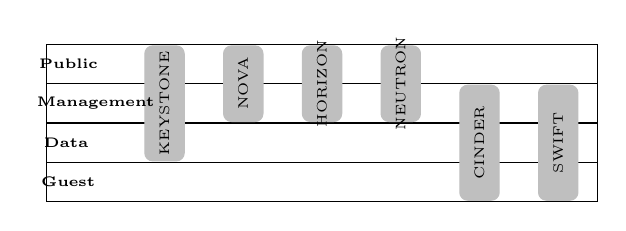
\begin{tikzpicture}
\draw [] (0,0) rectangle (7.,.5);
\draw [] (0,0.5) rectangle (7.,1);
\draw [] (0,1) rectangle (7.,1.5);
\draw [] (0,1.5) rectangle (7.,2);

\draw [rounded corners=1mm,fill=lightgray,color=lightgray] (1.25,.52) rectangle (1.75,1.98);
\draw [rounded corners=1mm,fill=lightgray,color=lightgray] (2.25,1.02) rectangle (2.75,1.98);
\draw [rounded corners=1mm,fill=lightgray,color=lightgray] (3.25,1.02) rectangle (3.75,1.98);
\draw [rounded corners=1mm,fill=lightgray,color=lightgray] (4.25,1.02) rectangle (4.75,1.98);
\draw [rounded corners=1mm,fill=lightgray,color=lightgray] (5.25,0.02) rectangle (5.75,1.48);
\draw [rounded corners=1mm,fill=lightgray,color=lightgray] (6.25,0.02) rectangle (6.75,1.48);

\node (l1) at (0.28,1.75) {\tiny\bf{Public}};
\node (l1) at (0.625,1.25) {\tiny\bf{Management}};
\node (l1) at (0.25,0.75) {\tiny\bf{Data}};
\node (l1) at (0.275,0.25) {\tiny\bf{Guest}};

\node (l1) at (1.5,1.25) [rotate=90] {\tiny{KEYSTONE}};
\node (l1) at (2.5,1.5) [rotate=90] {\tiny{NOVA}};
\node (l1) at (3.5,1.5) [rotate=90] {\tiny{HORIZON}};
\node (l1) at (4.5,1.5) [rotate=90] {\tiny{NEUTRON}};
\node (l1) at (5.5,.75) [rotate=90] {\tiny{CINDER}};
\node (l1) at (6.5,.75) [rotate=90] {\tiny{SWIFT}};

\end{tikzpicture}

}
  \caption{Domini di sicurezza e servizi di OpenStack\label{fig:OpenStackServiziDomini}}
\end{figure}

Ai fini della validazione del framework sono stati effettuati vari processi di certificazione separati, aventi come obiettivo diverse proprietà di sicurezza \cite{CertOpenstack}.
Per ogni processo è stata definita una fase di inizializzazione nella quale:
\begin{itemize}
\item Viene effettuato il setup dei driver di sonda in relazione al target da certificare.
\item Vengono sviluppati gli aggregatori per integrare i risultati dei test, affinché sia possibile rilasciare l'eventuale certificato.
\item Viene stabilito un \textit{ciclo di vita} del processo di certificazione, per gestire la validità del certificato una volta emesso \cite{CertOpenstack}.
\end{itemize}
Per ogni proprietà sono state descritte le attività svolte e i risultati ottenuti dettagliando:
\begin{itemize}
\item L'obiettivo dell'attività di test
\item Il target della certificazione, in termini di servizi OpenStack coinvolti
\item La definizione del test, specificando i casi di test più dettagliati
\item Un'analisi dei risultati ottenuti e dei costi aggiunti implicati dal processo di certificazione
\end{itemize}
Lo scopo non è quello di dimostrare l'assoluta sicurezza di OpenStack, quanto quello di fornire un insieme di casi di test e di prove che un'autorità di certificazione può considerare o meno sufficienti per rilasciare un certificato di sicurezza per questo software.

\subsection{Confidenzialità dei dati di autenticazione}

\paragraph{Obiettivo}
Questo test ha come obiettivo la valutazione della confidenzialità delle informazioni di autenticazione relative ad OpenStack.
A tale fine occorre:
\begin{enumerate}
\item Verificare che le credenziali siano conservate e gestite nel modo corretto
\item Assicurarsi che l'autenticazione avvenga tramite un canale cifrato: occorre che sia presente la cifratura TLS/SSL su tutti i canali di comunicazione, compreso l'endpoint della dashboard Horizon, affinché non sia possibile per un utente malintenzionato ottenere le credenziali effettuando operazioni di \textit{sniffing} del traffico o \textit{tampering}.
\item I dati siano disponibili solo per il reale proprietario: i file di configurazione contenenti eventuali credenziali in chiaro o chiavi devono essere protetti con meccanismi di controllo degli accessi, affinché siano consultabili e/o utilizzabili solamente dalle persone autorizzate.
\end{enumerate}
\paragraph{Target della certificazione}
Questo test insiste sui dominio di sicurezza \textit{pubblico} e di \textit{gestione} e include i servizi \textit{keystone}, \textit{nova}, \textit{neutron}, \textit{swift}, \textit{cinder}, \textit{glance} e \textit{horizon}. 
\paragraph{Definizione del test}
Al fine di verificare la proprietà ivi definita vengono utilizzati due casi di test:
\begin{itemize}
\item \textit{Valutazione del canale di comunicazione} utilizzato nello scambio delle credenziali. Ciò avviene tramite uno script \textit{LUA} per \textit{NMap} appositamente realizzato, in grado di ottenere le informazioni di cifratura per i canali di comunicazione (presenza e versioning di TLS/SSL, validità dei certificati, tecniche di hashing per le chiavi, cifrari supportati, eventuali vulnerabilità note, ad es. Heartbleed).

Pseudocodice:

\begin{python}
cond_SSLTLS = cond_chipers = cond_validity = False
[host, port, xml_file]= get_input()

execute("nmap -oX [xml_file] -p [PORT] --script ssl-cert-custom,ssl-enum-ciphers-custom [HOST]")
result = parse( xml_file )

cond_SSLTLS = https.isTLS(result)
if cond_SSLTLS is True:
    cond_validity = https.checkValidity(result)
    cond_chipers = https.isAllStrong(result)

return cond_validity and cond_chipers
\end{python}

\item \textit{Politiche per il controllo degli accessi} sui file contenenti le credenziali di autenticazione (es. file di configurazione dei servizi). 
Più specificatamente, il driver di sonda effettua il login sull'host target ripetutamente con varie credenziali valide specificate in input, verificando che siano impostati permessi sufficientemente restrittivi sui file in questione e che essi siano effettivamente applicati, tenendo anche conto dell'eventuale contesto SELinux in cui il file è collocato.

Pseudocodice:

\begin{python}
cond_owner = cond_group = cond_others = False

[owner_u, group_u, others_u, ssh_priv_key, file, privileges] = get_ input()

connection = ssh(owner_u, ssh_priv_key)
cond_owner = connection.checkWRE(file, privileges)

connection = ssh(group_u, ssh_priv_key)
cond_group = connection.checkWRE(file, privileges)

connection = ssh(other_u, ssh_priv_key)
cond_others = connection.checkWRE(file, privileges)

return cond_owner and cond_group and cond_others
\end{python}

Un'implementazione di questo driver di sonda è proposta in appendice.

\end{itemize}
\paragraph{Analisi dei risultati}
La proprietà viene certificata se e solo se entrambi i casi di test riportano un risultato positivo.
Poiché l'ambiente di test sul quale è stata effettuata la certificazione (basato su Devstack, configurato in modalità SSL nativa) è conforme alle linee guida OSSG, entrambi i casi di test hanno avuto risultato positivo e la proprietà è stata certificata.

\paragraph{Valutazione dei costi}
Sul nostro ambiente di test il processo di certificazione è stato eseguito in \textit{3.139 s} così suddivisi:
\begin{itemize}
\item Valutazione del canale di comunicazione: \textit{2.9282 s}, dovuto al costo della scansione NMap nei confronti del target. Questa operazione genera traffico di rete in quantità trascurabile.
\item Politiche per il controllo degli accessi: \textit{210 ms}, dovuto alle tre connessioni SSH implicate. Le operazioni coinvolte generano traffico di rete in quantità trascurabile, ed effettuano richieste al file system.
\end{itemize}

\subsection{Confidenzialità del block-storage}
Un'ulteriore proprietà fondamentale per la sicurezza nel cloud è costituita dalla sicurezza dei dati memorizzati dalle istanze, discussa nella tesi di Roberto Veca \cite{RobertoVeca}.
A tal fine Cinder e Nova supportano l'utilizzo di \textit{dm-crypt}, che consente la creazione di storage LUKS crittografati a livello di infrastruttura.
L'operazione di attachment di un volume cifrato può essere vista come una funzione \textit{attachment(volumeId,instanceId)} così strutturata:
\begin{itemize}
\item Cinder mette a disposizione, mediante un canale iSCSI, il volume \textit{volumeId}, ancora criptato, al nodo di Compute sul quale è ospitata la macchina \textit{instanceId}
\item Il servizio Nova ospitato sul nodo di Compute effettua, tramite \textit{dm-crypt}, la decifratura del volume e mette a disposizione il volume già in chiaro alla macchina virtuale.
\end{itemize}
Questa funzionalità di OpenStack fornisce un livello di cifratura completamente trasparente per il sistema operativo guest capace di evitare il problema della rimanenza del dato, tuttavia chiunque abbia accesso all'infrastruttura può tranquillamente accedere e modificare i dati: le chiavi di cifratura non sono gestite dal reale utilizzatore della macchina virtuale, ma dal gestore dell'infrastruttura.
\begin{figure}[H]
\centering
\makebox[\textwidth]{
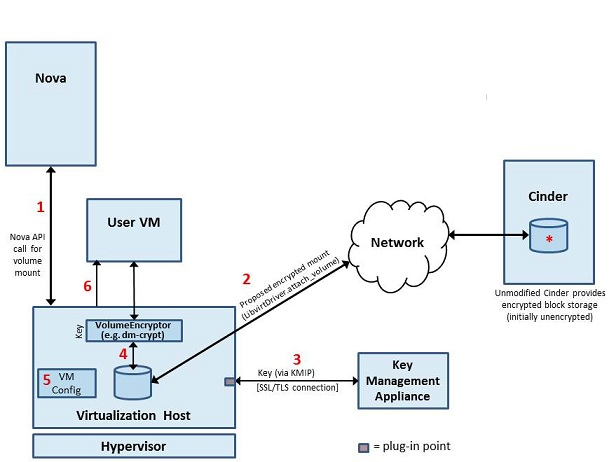
\includegraphics[width=\textwidth]{immagini/VolumeEncryption.png}
}
\caption{Workflow della cifratura dei volumi a blocchi su OpenStack \cite{OpenStackBlockEnc}}\label{VolumeEnc}
\end{figure}


\paragraph{Obiettivo}
L'obiettivo di questo processo di certificazione è quello di verificare che i dati memorizzati siano effettivamente memorizzati in modo sicuro e che non sia possibile ottenere il dato in chiaro effettuando l'analisi del volume cifrato.

\paragraph{Target della certificazione}
Questo test insiste sui dominio di sicurezza \textit{dati} e \textit{gestione} e include i servizi \textit{nova} e \textit{cinder}.
\paragraph{Definizione del test}

Questo processo di certificazione si basa su due casi di test:
\begin{itemize}
\item \textit{Verifica del comportamento del meccanismo di cifratura}. Questo caso di test è composto dalle seguenti fasi:
\begin{enumerate}
\item Creazione di un volume, chiamato "clean", non cifrato
\item Creazione di un volume, chiamato "luks", cifrato
\item Deploy di una macchina virtuale
\item Montaggio dei volumi sulla macchina virtuale
\item Iniezione di uno script all'interno della macchina virtuale con lo scopo di scrivere una frase di \textit{challenge} in entrambi i volumi
\item Smontaggio dei volumi
\item Analisi bit a bit dei volumi, a livello infrastruttura, alla ricerca della \textit{challenge} memorizzata dalla macchina virtuale
\end{enumerate}
Il test ha successo se e solo se la frase di \textit{challenge} sia leggibile esclusivamente sul volume chiamato "clean".

Pseudocodice:

\begin{python}

[challenge , instance_id, nova_address, cinder_address, cinder_user, ssh_priv_key] = get_input()

cinder = CinderClient(cinder_address)
nova = NovaClient(nova_address)

cinder.createVolumeType("LUKS")
stLuks = cinder.createVolume("LUKS")
stPlain = cinder.createVolume("PLAIN")
vm = nova.createVM()
vm.deploy()
vm.attachVolume(stClean)
vm.attachVolume(stLuks)
vm.injectScript(WriteChallenge)
vm.shutdown()

shell = connectionSSH(cinder_address, cinder_user , ssh_priv_key);
devMapLuks = shell.findDeviceMapVolume(stLuks)
devMapPlain = shell.findDeviceMapVolume(stPlain)

isChallengeL = shell.findString(challenge, devMapLuks)
isChallengeP = node.findString(challenge, devMapPlain)

return isChallengeC and not isChallengeL
\end{python}

\item \textit{Valutazione del trattamento dei dati successivamente all'\textit{attachment} del volume}. Questo caso di test viene eseguito parallelamente al primo e si occupa di valutare come i dati vengono trattati successivamente all'attachment del volume. All'atto pratico, controlla se i dati crittografati siano disponibili in chiaro a un amministratore dell'infrastruttura o ad altri utenti che eseguono attacchi di \textit{privilege escalation} o \textit{VM escaping}. Il test restituisce valutazioni differenti in base alla quantità di dati disponibili in chiaro.

Pseudocodice:

\begin{python}
[challenge , instance_id, nova_address, cinder_address, cinder_user, ssh_priv_key] = get_input()

cinder = CinderClient(cinder_address)
nova = NovaClient(nova_address)

cinder.createVolumeType("LUKS")
stLuks = cinder.createVolume("LUKS")

vm = nova.createVM()
vm.deploy()
vm.attachVolume(stLuks)
vm.injectScript(WriteChallenge)
vm.shutdown()

shell = connectionSSH(cinder_address, cinder_user, ssh_priv_key);
devMap = shell.findDeviceMapVolume(stLuks)
isChallengeL = shell.findString(challenge, devMap)
return not isChallengeL
\end{python}

\end{itemize}
\paragraph{Analisi dei risultati}
La proprietà di confidenzialità dello storage identifica tre livelli di certificazione:
\begin{enumerate}
\item Correttezza del meccanismo di protezione (livello 1), se e solo se i dati memorizzati nel volume crittografato sono leggibili soltanto in seguito a un'operazione di decifratura avvenuta in modo lecito
\item Cifratura e decifratura selettiva (livello 2), se e solo se, leggendo o scrivendo i dati memorizzati nel volume crittografato, sia stata effettuata un'operazione di decifratura lecita
\item Cifratura completa (livello 3). se e solo se i dati memorizzati nel volume cifrato non sono mai accessibili alle entità che non detengono la giusta chiave di decifratura
\end{enumerate}
Nell'ambiente di test, basato su Devstack, il primo caso di test ha avuto successo (è stato possibile individuare la \textit{challenge} a livello infrastruttura solamente nel volume in chiaro).
Il secondo caso di test, invece, ha avuto esito negativo in quanto l'implementazione di OpenStack, come descritto sopra, permette a un amministratore di infrastruttura di accedere ai dati in chiaro.
La proprietà quindi, non è stata certificata ai livelli 2 e 3.

\paragraph{Valutazione dei costi}
Sul nostro ambiente di test il processo di certificazione è stata eseguito in \textit{14.549 s}. La tempistica calcolata tiene conto dei ritardi dovuti alle prestazioni della rete di laboratorio.
Per questo processo di certificazione bisogna tenere conto dei costi derivanti dal deployment di un'istanza e dalla creazione di due volumi a blocchi.
La macchina virtuale utilizzata in fase di test è basata su un'immagine del sistema operativo minimale CirrOS, del peso di 12.6 MB, con \textit{flavor} \textit{m1.tiny}, che alloca:
\begin{itemize}
\item 2 GB RAM
\item 20 GB di storage effimero
\item 0 GB di storage a blocchi
\item 0 GB di swap
\end{itemize}

I volumi a blocchi creati sono di 1 GB ciascuno. La procedura di creazione dei volumi prevede l'azzeramento dello spazio ad essi allocato, con un costo in termini di operazioni di \textit{I/O} proporzionale alle caratteristiche del dispositivo di memorizzazione.
I requisiti specificati devono persistere per tutto il tempo di esecuzione del test.

\subsection{Isolamento delle reti virtuali e firewalling}
Un ulteriore aspetto di sicurezza, fondamentale per il cloud, è costituito dall'isolamento delle reti tra le macchine virtuali e il resto dell'infrastruttura.
La funzionalità di rete è offerta dal software Neutron il quale, tramite l'utilizzo di plugin collegati a servizi esterni, offre una virtualizzazione dei livelli \textit{data-link} e \textit{network} dello stack ISO/OSI (\textit{software-defined} network).
In particolare, nell'ambiente di test (il setup multinodo effettuato nel laboratorio Sesar), è stato utilizzato il plug-in per \textit{openVSwitch}.

Per fornire l'isolamento delle reti, Neutron dispone di una funzionalità chiamata \textit{security group}, la quale permette di definire dei domini di sicurezza tra le istanze, specificando la lista delle porte ammesse per la comunicazione dei servizi.
L'isolamento avviene in modo trasparente all'istanza, tramite \textit{iptables}. Tuttavia, la mancanza di un controllo di consistenza tra le regole specificate nei \textit{security group} e quelle specificate in \textit{iptables} lascia spazio ad attacchi che potrebbero avere luogo in caso di presenza di regole di firewalling ignote all'utente.

\paragraph{Obiettivo}
L'obiettivo di questo processo di certificazione è controllare che sia possibile effettuare traffico verso un'istanza solamente in base alle regole dichiarate nella definizione del \textit{security group}.

\paragraph{Target della certificazione}
I domini implicati sono \textit{pubblico} e \textit{Guest}, il servizio al quale si fa riferimento è Neutron.

\paragraph{Definizione del test}
Questo processo di certificazione prevede l'esecuzione di un solo caso di test così composto:
\begin{enumerate}
\item Deployment di un'istanza honeypot
\item Iniezione di uno script che apre le porte in un determinato intervallo sull'istanza honeypot mediante il comando \textit{netcat}
\item Associazione tra l'istanza e un \textit{security group} definito a priori
\item Dichiarazione di un floating ip e associazione dello stesso all'istanza
\item Rilevamento delle regole dichiarate nella definizione del \textit{security group}
\item Testing con \textit{nmap} dell'istanza
\item Confronto dei risultati della scansione \textit{nmap} con le regole del security group
\end{enumerate}

Pseudocodice:

\begin{python}
[image_id, sg, nova_address, neutron_address] = get_input()

nova = NovaClient(nova_address)
neutron = NeutronClient(neutron_address)
nmap = NMap()

virtual_machine = nova.createVM(image_id)
virtual_machine.injectScript(openAllPortsTCP)
virtual_machine.injectScript(openAllPortsUDP)
virtual_machine.assignSecurityGroup(sg)
vm_ip = neutron.declareFloatingIp()
virtual_machine.assignFloatingIp(vm_ip)

all_sgs = nova.getAllSecurityGroups(virtual_machine)
sgs_results = parseMultipleSecurityGroups(all_sgs)
nmap_results = nmap.scan(vm_ip)

return compare(sgs_results, nmap_results)
\end{python}

Un'implementazione del presente driver di sonda è fornita in appendice.

\paragraph{Analisi dei risultati}
La proprietà è certificata se e solo se le porte aperte individuate da \textit{nmap} sono un sottoinsieme di quelle definite nel \textit{security group}.
Nell'ambiente di test nel quale è stata effettuato il processo di certificazione abbiamo ottenuto un risultato positivo, constatando la coerenza tra quanto dichiarato nel \textit{security group} e quanto effettivamente applicato a livello di rete.

\paragraph{Valutazione dei costi}

Sul nostro ambiente di test il processo di certificazione è stata eseguito in \textit{23.714 s}.
Questo intervallo di tempo comprende:
\begin{itemize}
\item Deployment della macchina virtuale, associazione del \textit{security group} e del \textit{floating ip}, apertura delle porte TCP nell'intervallo \textit{1-65535} (8.263 s)
\item Lettura delle informazioni su tutti i \textit{security groups} associati all'istanza (2.738 s)
\item Scansione dell'istanza con \textit{nmap} (12.701 s)
\item Confronto dei risultati con le regole del \textit{security group} (0.012 s)
\end{itemize}
Nella presente valutazione è stata presa in considerazione solamente l'analisi delle porte TCP e la scansione con nmap è stata effettuata in modalità \textit{connect scan}.
Il driver di sonda sviluppato consente di effettuare una scansione più granulare con \textit{SYN scan}, il ché potrebbe comportare un aumento notevole del tempo di scansione.
L'analisi delle porte UDP, inoltre, richiede tempistiche ancora maggiori.
Le tempistiche valutate inglobano i tempi di risposta dei servizi dell'ambiente di test.
L'istanza utilizzata è basata su un'immagine del sistema operativo Ubuntu, del peso di 244 MB, con flavor personalizzato che alloca:
\begin{itemize}
\item 512 MB RAM
\item 1 GB di storage effimero
\end{itemize}

\end{document}
